\chapter{التخليق اللاتناظري}\label{ch:b3:asymmetric-synthesis}

كان الليفودوبا، الدواء الذي يخفف أعراض داء باركنسون، في
السبعينيات أول مركب يُصنع صناعيًا \omterm{def:b3:asymmetric-synthesis:asymmetric-catalysis}{بالحفز اللاتناظري}: فبضعة
غرامات من معقد روديوم كيرالي، مذابة مع طليعة مستوية لاكيرالية
تحت الهيدروجين، أعطت ناتجًا يفوق فيه أحد المتماكبين المرآويين
الآخرَ عددًا بكثير. وقد يختلف المتماكبان المرآويان لدواء اختلافًا تامًا في آثارهما،
لأن المستقبلات والإنزيمات التي يلاقيانها هي نفسها كيرالية. ويقيس هذا
الفصل النقاوة المرآوية، ويفسّر كيف يختار محيط كيرالي
بين طريقين متناظرين مرآويًا، ويستعرض الاستراتيجيات (\omterm{def:b3:asymmetric-synthesis:chiral-pool}{المخزون الكيرالي}،
والمساعدات، والفصل، والحفازات الفلزية والعضوية) التي تصنع متماكبات مرآوية
مفردة.

\begin{recall}
عرّف مجلد السنة الأولى الكيرالية، والمتماكبات المرآوية، والمتماكبات اللامرآوية، والخلائط
الراسيمية، والدوران النوعي، وقواعد CIP والتفاعلات الانتقائية فراغيًا 
والنوعية فراغيًا؛ وعرّف مجلد السنة الثانية الهدرجة الحفزية،
والإيبوكسدة، والهيدروكسلة الثنائية، والإيمينات، والإينامينات، والإينولات، والتفاعل الألدولي،
وحلقنة روبنسون والكروماتوغرافيا. وأعطى \cref{ch:b3:rate-theories}
\omterm{thm:b3:rate-theories:eyring}{معادلة أيرنغ}، و\cref{ch:b3:homogeneous-catalysis} دورة ويلكنسون، 
و\cref{ch:b3:point-groups} المحور $C_2$.
\end{recall}

\begin{omfigure}
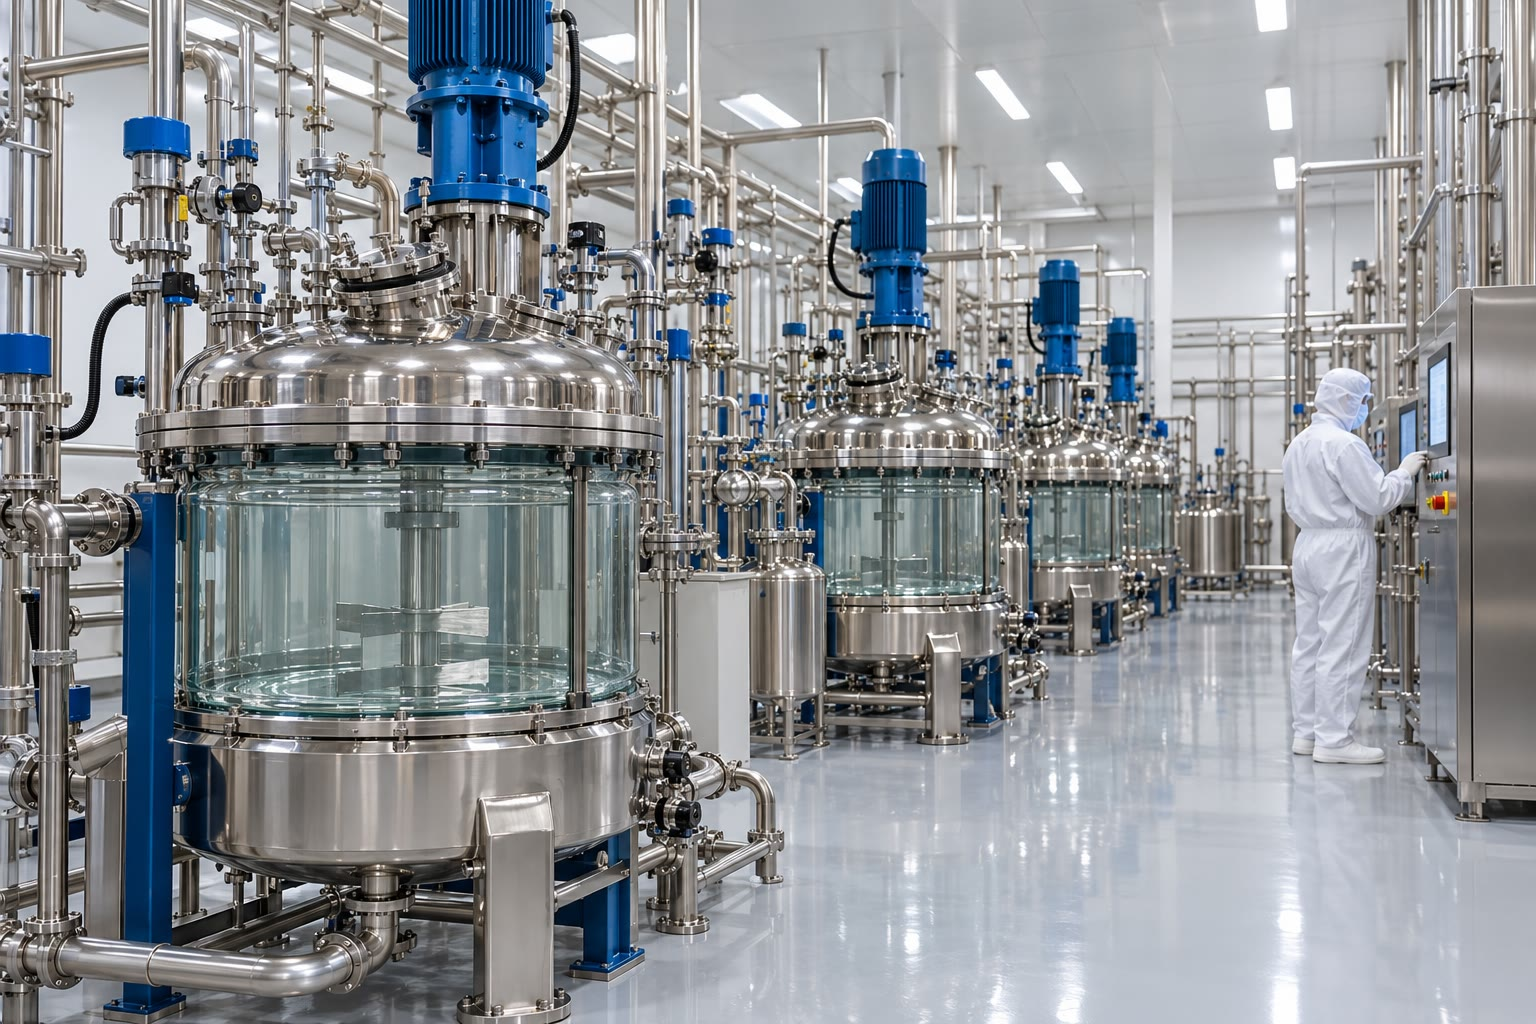
\includegraphics[width=0.58\linewidth]{images/book4/ai/b3-28-api-plant.jpg}

{\small قاعة مفاعلات مبطنة بالزجاج في مصنع لإنتاج المكوّنات الصيدلانية
الفعالة. كثير من منتجاته متماكبات مرآوية مفردة، تُصنع
بالحفز أو بالفصل وتُفحص بالكروماتوغرافيا الكيرالية.}
\end{omfigure}

\section{قياس النقاوة المرآوية}

\begin{definition}[الزيادة المرآوية]\label{def:b3:asymmetric-synthesis:ee}
من أجل خليط من متماكبين مرآويين بكميتين $n_R \ge n_S$، تكون \emph{الزيادة
المرآوية}\index{زيادة مرآوية} هي $\mathrm{ee} = (n_R - n_S)/(n_R + n_S)$ و\emph{النسبة المرآوية}
\index{نسبة مرآوية} $\mathrm{er} = n_R/n_S$؛ ومن أجل المتماكبات اللامرآوية، تُعرَّف
\emph{الزيادة اللامرآوية}\index{زيادة لامرآوية} de بالطريقة
نفسها. و\emph{النقاوة الضوئية}\index{نقاوة ضوئية} هي نسبة
الدوران النوعي لعيّنة إلى الدوران النوعي للمتماكب المرآوي النقي.
\end{definition}

\begin{proposition}[ee وer]\label{prop:b3:asymmetric-synthesis:ee-er}
$\mathrm{ee} = (\mathrm{er} - 1)/(\mathrm{er} + 1)$ و$\mathrm{er} = (1 + \mathrm{ee})/(1 - \mathrm{ee})$.
\end{proposition}

\begin{proof}
اقسم بسط $(n_R - n_S)/(n_R + n_S)$ ومقامه على $n_S$؛ والحل بالنسبة إلى er يعطي
الصيغة الثانية.
\end{proof}

\omterm{def:b3:asymmetric-synthesis:ee}{الزيادة المرآوية} 90\,\% تقابل \omterm{def:b3:asymmetric-synthesis:ee}{نسبة مرآوية} 95\,:\,5، والزيادة 98\,\% تقابل نسبة 99\,:\,1. ولا تساوي \omterm{def:b3:asymmetric-synthesis:ee}{النقاوة الضوئية}
الزيادةَ المرآوية إلا إذا كان الدوران متناسبًا مع التركيب؛ والشوائب، 
والمذيب، وآثار التركيز، وصغر دوران مركبات كثيرة تجعلها
غير موثوقة، فتُقاس \omterm{def:b3:asymmetric-synthesis:ee}{الزيادة المرآوية} بفصل المتماكبين المرآويين.

\begin{method}[الزيادة المرآوية من كروماتوغرام كيرالي]\label{met:b3:asymmetric-synthesis:ee-chromatogram}
\begin{enumerate}
  \item احقن الخليط الراسيمي أولًا، لتعرف القمتين وتتحقق من
        انفصالهما (فصل حتى خط الأساس) وتساوي مساحتيهما.
  \item احقن العيّنة وكامِل القمتين.
  \item للمتماكبين المرآويين الاستجابة نفسها في كاشف لاكيرالي، ومنه
        $\mathrm{ee} = (A_1 - A_2)/(A_1 + A_2)$؛ وأسند القمتين بمرجع نقي مرآويًا.
\end{enumerate}
\end{method}

\begin{omfigure}
\begin{tikzpicture}
\begin{axis}[name=a, width=0.48\linewidth, height=5.4cm, xmin=0, xmax=20, ymin=0, ymax=1.0,
  axis lines=left, xlabel={\babelsublr{$\Delta\Delta G^\ddagger$ / \unit{kJ.mol^{-1}}}}, ylabel={\babelsublr{ee}},
  tick label style={font=\scriptsize}, label style={font=\small}]
\addplot[omDef, thick] table[x=ddg, y=eeA] {figdata/out/bachelor-3-er-ddg.dat};
\addplot[omMeth, thick] table[x=ddg, y=eeB] {figdata/out/bachelor-3-er-ddg.dat};
\addplot[omThm, thick] table[x=ddg, y=eeC] {figdata/out/bachelor-3-er-ddg.dat};
\node[font=\scriptsize, omDef, anchor=west] at (axis cs:10,0.55) {\qty{-78}{\celsius}};
\node[font=\scriptsize, omMeth, anchor=west] at (axis cs:10,0.43) {\qty{0}{\celsius}};
\node[font=\scriptsize, omThm, anchor=west] at (axis cs:10,0.31) {\foreignlanguage{arabic}{\babelsublr{\qty{25}{\celsius}}، المنحنى الأدنى}};
\end{axis}
\begin{axis}[at={(a.east)}, anchor=west, xshift=1.4cm, width=0.48\linewidth, height=5.4cm,
  xmin=7.5, xmax=9.5, ymin=0, axis lines=left, ytick=\empty,
  xlabel={\foreignlanguage{arabic}{زمن الاستبقاء \babelsublr{(min)}}}, ylabel={\foreignlanguage{arabic}{إشارة الكاشف}},
  tick label style={font=\scriptsize}, label style={font=\small}]
\addplot[black, thick] table[x=t, y=y] {figdata/out/bachelor-3-er-ddg-b.dat};
\node[font=\scriptsize, anchor=south west] at (axis cs:8.3,250) {(\textit{R}): 97.5};
\node[font=\scriptsize, anchor=south] at (axis cs:9.1,20) {(\textit{S}): 2.5};
\end{axis}
\end{tikzpicture}

{\small يسارًا: \omterm{def:b3:asymmetric-synthesis:ee}{الزيادة المرآوية} بدلالة الفرق في \omterm{def:b3:rate-theories:activation}{طاقة جيبس
للتنشيط} بين الطريقين المتنافسين، عند ثلاث درجات حرارة: فالقيمة نفسها للفرق
$\Delta\Delta G^\ddagger$ تعطي \omterm{def:b3:asymmetric-synthesis:ee}{زيادة مرآوية} أعلى عند درجة الحرارة المنخفضة. يمينًا: كروماتوغرام HPLC كيرالي،
مساحتا القمتين 97.5 و2.5 (نموذج): \omterm{def:b3:asymmetric-synthesis:ee}{الزيادة المرآوية} 95\,\%.}
\end{omfigure}

لا يميّز الرنين المغناطيسي النووي بين المتماكبين المرآويين إلا في محيط كيرالي: فعامل الإذابة
الكيرالي يكوّن معقدات لامرآوية قصيرة العمر تختلف إشاراتها، 
والكحول أو الأمين الكيرالي المحوَّل إلى إستريه اللامرآويين مع
حمض موشر يكشف التشكيل من نمط فروق الانزياح.

\begin{method}[التشكيل من إسترات موشر، بإيجاز]\label{met:b3:asymmetric-synthesis:mosher}
\begin{enumerate}
  \item اصنع إستري MTPA كليهما، (\textit{R}) و(\textit{S})، للكحول.
  \item سجّل طيفيهما البروتونيين واحسب $\Delta\delta = \delta_S - \delta_R$ للبروتونات على كل
        جانب من كربون الكاربينول.
  \item في التشكُّل المفضل تحجب حلقة الفينيل في الحمض جانبًا واحدًا:
        فالبروتونات ذات $\Delta\delta > 0$ تقع في جانب، وذات $\Delta\delta < 0$ في الجانب الآخر، وهذا
        يحدد موضع المستبدلين ويعطي التشكيل.
\end{enumerate}
\end{method}

\section{الموضعية والإضافات الانتقائية فراغيًا}

\begin{definition}[التفاعلات الانتقائية فراغيًا]\label{def:b3:asymmetric-synthesis:selective}
\emph{التفاعل الانتقائي للمتماكبات المرآوية}\index{تفاعل انتقائي للمتماكبات المرآوية} يكوّن أحد
المتماكبين المرآويين لناتج بزيادة على الآخر؛ و\emph{التفاعل الانتقائي للمتماكبات
اللامرآوية}\index{تفاعل انتقائي للمتماكبات اللامرآوية} يكوّن متماكبًا لامرآويًا واحدًا بزيادة.
\end{definition}

\begin{definition}[الموضعية]\label{def:b3:asymmetric-synthesis:topicity}
تكون مجموعتان في جزيء \emph{متكافئتي الموضع}\index{متكافئ الموضع} حين يبادل بينهما
دوران للجزيء (فاستبدال أي منهما يعطي المركب نفسه)،
و\emph{مرآويتي الموضع}\index{مرآوي الموضع} حين لا يبادل بينهما إلا انعكاس
(فاستبدال إحداهما أو الأخرى يعطي متماكبين مرآويين)، 
و\emph{لامرآويتي الموضع}\index{لامرآوي الموضع} حين لا تبادل بينهما أي \omterm{def:b3:point-groups:operation}{عملية تناظر}
(فاستبدال إحداهما أو الأخرى يعطي متماكبين لامرآويين).
\end{definition}

ذرتا الهيدروجين في مجموعة $\ce{CH2}$ مجاورة لمركز فراغي \omterm{def:b3:asymmetric-synthesis:topicity}{لامرآويتا الموضع}: فلهما
انزياحان كيميائيان مختلفان وتقترنان إحداهما بالأخرى، ولهذا تظهر مثل هذه
المجموعة غالبًا في صورة إشارتين في الرنين المغناطيسي النووي.

\begin{definition}[الأوجه السابقة للكيرالية]\label{def:b3:asymmetric-synthesis:faces}
ذرة الكربون المثلثية ذات المستبدلات الثلاثة المختلفة \emph{سابقة للكيرالية}\index{سابق للكيرالية}:
فإضافة مجموعة رابعة مختلفة تُنشئ مركزًا فراغيًا. ووجهها الذي تبدو فيه
المستبدلات الثلاثة بترتيب أولوية CIP المتناقص دائرةً مع عقارب الساعة هو
\emph{الوجه Re}\index{وجه Re}؛ وعكس عقارب الساعة، \emph{الوجه Si}\index{وجه Si}.
\end{definition}

\begin{omfigure}
\begin{tikzpicture}[font=\small, >=Stealth]
  \coordinate (c) at (0,0);
  \draw[thick, double, double distance=1.6pt] (c) -- (90:1.1) node[above] {O (1)};
  \draw[thick] (c) -- (210:1.1) node[below left] {$\ce{C6H5}$ (2)};
  \draw[thick] (c) -- (330:1.1) node[below right] {$\ce{CH3}$ (3)};
  \fill (c) circle (1.6pt);
  \draw[->, thick, omThm] (70:0.6) arc[start angle=70, end angle=200, radius=0.6];
  \node[font=\scriptsize, omThm, align=center] at (-1.9,0.75) {1 $\to$ 2 $\to$ 3\\ \foreignlanguage{arabic}{عكس عقارب الساعة:}\\ \foreignlanguage{arabic}{الوجه \textit{Si}}};
  \node[font=\scriptsize, align=left, anchor=west] at (2.6,0.4) {\foreignlanguage{arabic}{الوجه المقابل للقارئ: \textit{Si}}\\ \foreignlanguage{arabic}{الوجه خلف الصفحة: \textit{Re}}};
  \node[font=\scriptsize, align=left, anchor=west] at (2.6,-0.5) {\foreignlanguage{arabic}{الهيدريد المضاف من الوجه \textit{Re}}\\ \foreignlanguage{arabic}{يعطي \babelsublr{(\textit{S})}-1-فينيل إيثانول}};
\end{tikzpicture}

{\small وجها الأسيتوفينون. من الأمام، تدور مستبدلات
كربون الكربونيل بترتيب CIP (O، الفينيل، الميثيل) عكس عقارب الساعة: فالوجه الأمامي
هو \textit{Si}، والوجه الخلفي \textit{Re}.}
\end{omfigure}

\begin{method}[إسناد الوجهين Re وSi]\label{met:b3:asymmetric-synthesis:re-si}
\begin{enumerate}
  \item رتّب المستبدلات الثلاثة للذرة المثلثية بقواعد CIP (فالرابطة
        المضاعفة تعدّ شريكها مرتين).
  \item انظر إلى الوجه المعني، والمستوي المثلثي في مستوي الصفحة.
  \item مع عقارب الساعة 1 $\to$ 2 $\to$ 3: \textit{Re}؛ وعكسها: \textit{Si}.
  \item لتسمية الناتج، أضف المجموعة الجديدة نحو الناظر وطبّق
        قواعد CIP على المركز الفراغي الجديد؛ فالهجوم من \omterm{def:b3:asymmetric-synthesis:faces}{الوجه Re} لا يعطي \textit{R} دائمًا.
\end{enumerate}
\end{method}

\begin{definition}[نموذج فلكين--آن والتحكم بالاستخلاب]\label{def:b3:asymmetric-synthesis:felkin}
\emph{نموذج فلكين--آن}\index{نموذج فلكين--آن} يتنبأ بالمتماكب اللامرآوي
الرئيس لإضافة محبة للنواة إلى مجموعة كربونيل مجاورة لمركز
فراغي: تقع أكبر مجموعة على ذلك المركز عمودية على مستوي
الكربونيل، ويقترب المحب للنواة في وضع anti منها، مارًّا بجانب أصغر
مجموعة، على امتداد مسار بورغي--دونيتز. وفي \emph{التحكم
بالاستخلاب}\index{تحكم بالاستخلاب}، يثبّت أيون فلزي مرتبط بأكسجين الكربونيل
وبمجموعة مانحة على المركز الفراغي التشكُّلَ، فيُضاف
المحب للنواة إلى الوجه الأقل إعاقة من حلقة الاستخلاب.
\end{definition}

\begin{proposition}[انتقائية فلكين--آن]\label{prop:b3:asymmetric-synthesis:felkin}
من أجل ألدهيد أو كيتون كيرالي عند الموضع $\alpha$ دون مجموعة مخلبية، يكون الناتج
الرئيس هو الذي يتنبأ به \omterm{def:b3:asymmetric-synthesis:felkin}{نموذج فلكين--آن} (وهو نموذج تجريبي،
تدعمه الحسابات). \admitted
\end{proposition}

\begin{omfigure}
\begin{tikzpicture}[font=\small, >=Stealth]
  \foreach \a/\lab in {90/L, 330/M, 210/S} {
    \draw[line width=0.8pt] (\a:0.55) -- (\a:1.1) node[pos=1.3] {\lab};
  }
  \fill[white] (0,0) circle (0.55);
  \draw[line width=0.8pt] (0,0) circle (0.55);
  \draw[line width=0.8pt, double, double distance=1.4pt] (0,0) -- (0:1.1) node[right] {O};
  \draw[line width=0.8pt] (0,0) -- (180:1.1) node[left] {R};
  \draw[->, very thick, omThm] (250:2.2) -- (250:0.25);
  \node[omThm, anchor=north] at (250:2.25) {Nu$^-$};
  \node[font=\scriptsize, align=left, anchor=west] at (1.7,-1.0) {\foreignlanguage{arabic}{يدخل \babelsublr{Nu$^-$} في وضع anti من L،}\\ \foreignlanguage{arabic}{مارًّا بجانب S، بزاوية نحو 107°}\\ \foreignlanguage{arabic}{مع الرابطة C=O}};
\end{tikzpicture}

{\small \omterm{def:b3:asymmetric-synthesis:felkin}{نموذج فلكين--آن}، كما يُرى على امتداد الرابطة من كربون الكربونيل (في الأمام،
الرابطتان إلى O وR) إلى المركز الفراغي (الدائرة الخلفية، المجموعات L وM وS). 
والمجموعة الكبيرة عمودية على مستوي الكربونيل؛ ويأتي المحب للنواة من
الجهة المقابلة، قريبًا من المجموعة الصغيرة وبعيدًا عن الأكسجين.}
\end{omfigure}

\section{الاستراتيجيات}

\begin{definition}[المخزون الكيرالي]\label{def:b3:asymmetric-synthesis:chiral-pool}
\emph{المخزون الكيرالي}\index{مخزون كيرالي} هو مجموعة المركبات الطبيعية
الرخيصة النقية مرآويًا (الأحماض الأمينية، والسكريات، والتربينات، والأحماض الهيدروكسيلية) المستعملة
مواد انطلاق، تُحمل مراكزها الفراغية إلى الهدف.
\end{definition}

\begin{definition}[المساعد الكيرالي]\label{def:b3:asymmetric-synthesis:auxiliary}
\emph{المساعد الكيرالي}\index{مساعد كيرالي} مجموعة نقية مرآويًا
تُربط مؤقتًا بركيزة للتحكم في الكيمياء الفراغية لتفاعل،
ثم تُزال وتُستعاد.
\end{definition}

في ألكلات إيفانز، يُؤسيَل أوكسازوليدينون مصنوع من حمض أميني؛
ويهاجم هاليدُ ألكيل إينولاتَ الليثيوم أو الصوديوم، المخلوب مع مجموعة كربونيل المساعد،
على الوجه البعيد عن مستبدل المساعد،
فيعطي متماكبًا لامرآويًا واحدًا، \omterm{def:b3:asymmetric-synthesis:ee}{بزيادة لامرآوية} تتجاوز غالبًا 95\,\%؛ ثم تحرر الحلمأة
الحمض الكيرالي والمساعد.

\begin{definition}[الفصل]\label{def:b3:asymmetric-synthesis:resolution}
\emph{فصل الخليط الراسيمي}\index{فصل الخليط الراسيمي} هو
فصله إلى متماكبيه المرآويين، تقليديًا ببلورة أملاح لامرآوية
مع حمض أو قاعدة نقية مرآويًا. وفي \emph{الفصل الحركي}\index{فصل حركي}
يتفاعل المتماكبان المرآويان بسرعتين مختلفتين مع كاشف أو حفاز كيرالي،
بانتقائية $s = k_{\mathrm{fast}}/k_{\mathrm{slow}}$. وفي \emph{الفصل الحركي
الديناميكي}\index{فصل حركي ديناميكي} يتحول المتماكبان المرآويان للركيزة
أحدهما إلى الآخر بسرعة بينما يتفاعل أحدهما.
\end{definition}

\begin{theorem}[معادلة كاغان]\label{thm:b3:asymmetric-synthesis:kagan}
في \omterm{def:b3:asymmetric-synthesis:resolution}{فصل حركي} لخليط راسيمي بتفاعلات من الرتبة الأولى انتقائيتها $s$،
يرتبط التحويل $c$ \omterm{def:b3:asymmetric-synthesis:ee}{والزيادة المرآوية} للركيزة الباقية بالعلاقة
\[
  s = \frac{\ln[(1 - c)(1 - \mathrm{ee})]}{\ln[(1 - c)(1 + \mathrm{ee})]}.
\]
\end{theorem}

\begin{proof}
يتناقص كل متماكب مرآوي أسيًا: فالنسبتان الباقيتان $f_1 = \eu^{-k_{\mathrm{fast}}t}$ 
و$f_2 = \eu^{-k_{\mathrm{slow}}t}$، ومنه $\ln f_1 = s\ln f_2$. وانطلاقًا من كميتين متساويتين، $1 - c = (f_1 + f_2)/2$ 
و$\mathrm{ee} = (f_2 - f_1)/(f_1 + f_2)$. ثم $(1 - c)(1 - \mathrm{ee}) = \tfrac12(f_1 + f_2)\cdot 2f_1/(f_1 + f_2) = f_1$ وكذلك
$(1 - c)(1 + \mathrm{ee}) = f_2$. ومنه $s = \ln f_1/\ln f_2$ هي النسبة المذكورة.
\end{proof}

\begin{omfigure}
\begin{tikzpicture}
\begin{axis}[width=0.62\linewidth, height=5.6cm, xmin=0, xmax=1, ymin=0, ymax=1.02,
  axis lines=left, xlabel={\foreignlanguage{arabic}{التحويل $c$}}, ylabel={\babelsublr{ee}},
  tick label style={font=\scriptsize}, label style={font=\small},
  legend style={font=\scriptsize, draw=none, at={(1.04,0.5)}, anchor=west}, legend cell align=left]
\addplot[color=omThm, thick] table[x=c, y=eesm] {figdata/out/bachelor-3-kinetic-resolution-s2.dat};
\addlegendentry{$s = 2$}
\addplot[color=omMeth, thick] table[x=c, y=eesm] {figdata/out/bachelor-3-kinetic-resolution-s10.dat};
\addlegendentry{$s = 10$}
\addplot[color=omDef, thick] table[x=c, y=eesm] {figdata/out/bachelor-3-kinetic-resolution-s50.dat};
\addlegendentry{$s = 50$}
\addplot[color=omThm, thick, dashed] table[x=c, y=eep] {figdata/out/bachelor-3-kinetic-resolution-s2.dat};
\addplot[color=omMeth, thick, dashed] table[x=c, y=eep] {figdata/out/bachelor-3-kinetic-resolution-s10.dat};
\addplot[color=omDef, thick, dashed] table[x=c, y=eep] {figdata/out/bachelor-3-kinetic-resolution-s50.dat};
\end{axis}
\end{tikzpicture}

{\small \omterm{def:b3:asymmetric-synthesis:resolution}{الفصل الحركي}: \omterm{def:b3:asymmetric-synthesis:ee}{الزيادة المرآوية} للركيزة الباقية (الخط المتصل) 
وللناتج (المتقطع) بدلالة التحويل، من أجل ثلاث انتقائيات. يمكن دائمًا جعل الركيزة
نقية مرآويًا بالمضي بعيدًا بما يكفي، على حساب المردود؛ أما
الناتج فيكون أنقى ما يكون عند تحويل ضعيف.}
\end{omfigure}

\begin{proposition}[الفصل الحركي الديناميكي]\label{prop:b3:asymmetric-synthesis:dkr}
إذا تحول المتماكبان المرآويان للركيزة أحدهما إلى الآخر أسرع بكثير من تفاعل أي منهما، أمكن
تحويل الخليط الراسيمي كله إلى متماكب مرآوي واحد للناتج، \omterm{def:b3:asymmetric-synthesis:ee}{بزيادة مرآوية} تحددها $s$:
$\mathrm{er} = s$.
\end{proposition}

\begin{proof}
يُبقي التراسم السريع المتماكبين المرآويين للركيزة بكميتين متساويتين في كل
لحظة. فتتكوّن النواتج بسرعتين نسبتهما $k_{\mathrm{fast}}[\mathrm A] : k_{\mathrm{slow}}[\mathrm A] = s$، ولا شيء
يوقف التفاعل قبل أن تُستهلك الركيزة كلها، عبر المتماكب السريع أساسًا:
فيمكن أن يبلغ المردود 100\,\% مع $\mathrm{er} = s$.
\end{proof}

\begin{method}[اختيار استراتيجية]\label{met:b3:asymmetric-synthesis:strategy}
\begin{enumerate}
  \item إذا كانت المراكز الفراغية للهدف موجودة في مركب طبيعي رخيص، فانطلق
        من \omterm{def:b3:asymmetric-synthesis:chiral-pool}{المخزون الكيرالي}.
  \item من أجل تخليق لمرة واحدة، أو لتثبيت مركز بموثوقية بجوار مجموعة
        كربونيل، استعمل مساعدًا، على حساب خطوتين إضافيتين.
  \item إذا كان الخليط الراسيمي رخيصًا وكان المتماكب غير المرغوب فيه قابلًا لإعادة التدوير أو
        التراسم، فافصله (تقليديًا، أو حركيًا أو ديناميكيًا).
  \item على النطاق الواسع، ابحث عن حفاز لاتناظري: مركز فراغي واحد يُصنع
        في كل دورة حفزية، دون نفايات كيرالية بكميات ستوكيومترية.
\end{enumerate}
\end{method}

\section{الحفز اللاتناظري بالفلزات}

\begin{definition}[الحفز اللاتناظري]\label{def:b3:asymmetric-synthesis:asymmetric-catalysis}
\emph{الحفز اللاتناظري}\index{حفز لاتناظري} تخليق انتقائي للمتماكبات المرآوية
بحفاز كيرالي يُستعمل بكمية صغيرة؛ وفي الحفازات الفلزية، تأتي
الكيرالية عادة من \emph{ربيطة كيرالية}\index{ربيطة كيرالية}.
\end{definition}

\begin{theorem}[الانتقائية من الطاقة]\label{thm:b3:asymmetric-synthesis:er-ddg}
إذا تكوّن ناتجان متماكبان مرآويًا عبر حالتين انتقاليتين لامرآويتين
بعاملين قبليين متساويين، تكوّنًا غير عكوس، تحت تحكم حركي، فإن
$\mathrm{er} = \exp(\Delta\Delta G^\ddagger/RT)$، حيث $\Delta\Delta G^\ddagger$ الفرق بين طاقتي جيبس
لتنشيطهما.
\end{theorem}

\begin{proof}
بحسب \omterm{thm:b3:rate-theories:eyring}{معادلة أيرنغ} (\cref{ch:b3:rate-theories})،
$k_i = (k_BT/h)\eu^{-\Delta G_i^\ddagger/RT}$؛ ويتكوّن الناتجان كلاهما من المتفاعلات نفسها، فتكون في كل لحظة
نسبة سرعتيهما $k_1/k_2 = \eu^{(\Delta G_2^\ddagger - \Delta G_1^\ddagger)/RT}$، وكذلك نسبة الكميتين المتكوّنتين.
\end{proof}

عند \qty{25}{\celsius} تحتاج \omterm{def:b3:asymmetric-synthesis:ee}{زيادة مرآوية} قدرها 99\,\% (\omterm{def:b3:asymmetric-synthesis:ee}{نسبة مرآوية} 199) إلى $\Delta\Delta G^\ddagger = RT\ln 199 = \qty{13.1}{kJ/mol}$، أي نحو طاقة
رابطة هيدروجينية واحدة؛ وعند \qty{-78}{\celsius} يكفي \qty{8.6}{kJ/mol}.

\begin{proposition}[الربائط ذات التناظر $C_2$]\label{prop:b3:asymmetric-synthesis:c2}
\omterm{def:b3:asymmetric-synthesis:asymmetric-catalysis}{الربيطة الكيرالية} ذات التناظر $C_2$ تنصّف عدد الحالات الانتقالية اللامرآوية
التي يجب مقارنتها، لأن موقعي التناسق اللذين تتركهما
متكافئان.
\end{proposition}

\begin{proof}
الدوران $C_2$ للحفاز ينقل أحد الموقعين الحرين إلى الآخر ويترك
الحفاز دون تغيير؛ فكل حالة انتقالية عند أحد الموقعين مطابقة إذن
لنظيرتها المدوَّرة عند الآخر. فلا تلزم مقارنة إلا أنماط الارتباط عند موقع واحد (وجه الركيزة،
واتجاهها).
\end{proof}

استعمل نولز فوسفينات أحادية كيرالية، ثم ثنائي الفوسفين DIPAMP ذا التناظر $C_2$، مع الروديوم
لهدرجة إيناميد إلى الحمض الأميني المحمي في الليفودوبا؛ ويهدرج BINAP لنويوري،
مع الروثينيوم، الكيتونات والألكينات الموظَّفة، ويهدرج،
مع ثنائي أمين كيرالي، الكيتونات البسيطة \omterm{def:b3:asymmetric-synthesis:ee}{بزيادة مرآوية} مرتفعة جدًا. وفي
هدرجة الإيناميد بالروديوم يأتي الناتج الرئيس من معقد الحفاز--الركيزة
الأقل استقرارًا والأقل وفرة، الذي يتفاعل مع الهيدروجين أسرع بكثير: فتتحدد
الانتقائية عند الحالات الانتقالية، لا بأعداد
الوسائط (مبدأ كيرتن--هاميت).

\begin{definition}[إيبوكسدة شاربلس]\label{def:b3:asymmetric-synthesis:sharpless}
\emph{إيبوكسدة شاربلس}\index{إيبوكسدة شاربلس} هي
الإيبوكسدة الانتقائية للمتماكبات المرآوية للكحولات الأليلية بهيدروبيروكسيد \textit{tert}-بوتيل،
بحفز إيزوبروبوكسيد التيتانيوم(IV) مع طرطرات ثنائي الإيثيل النقية مرآويًا؛ إذ يرتبط
الكحول بالتيتانيوم، الذي يوصل الأكسجين إلى أحد وجهي
الألكين، الذي تختاره الطرطرات.
\end{definition}

\begin{omfigure}
\begin{tikzpicture}[font=\small, >=Stealth]
  \draw[black!50] (-2.3,-1.55) rectangle (2.5,1.55);
  % C3 (top) = C2 (bottom); C2 carries R1 (left) and CH2OH (lower right),
  % C3 carries R2 (left) and R3 (right)
  \coordinate (c3) at (0,0.45); \coordinate (c2) at (0,-0.45);
  \draw[thick, double, double distance=1.6pt] (c3) -- (c2);
  \draw[thick] (c3) -- (-0.9,0.95) node[above left, inner sep=1pt] {R$^2$};
  \draw[thick] (c3) -- (0.9,0.95) node[above right, inner sep=1pt] {R$^3$};
  \draw[thick] (c2) -- (-0.9,-0.95) node[below left, inner sep=1pt] {R$^1$};
  \draw[thick] (c2) -- (0.9,-0.95) node[below right, inner sep=1pt] {$\ce{CH2OH}$};
  \draw[->, very thick, omDef] (0.35,2.5) -- (0.2,0.1) node[pos=0, above, align=center, font=\scriptsize] {\foreignlanguage{arabic}{\babelsublr{D-($-$)}-طرطرات ثنائي الإيثيل:}\\ \foreignlanguage{arabic}{O من الوجه العلوي}};
  \draw[->, very thick, omThm] (0.35,-2.6) -- (0.2,-0.1) node[pos=0, below, align=center, font=\scriptsize] {\foreignlanguage{arabic}{\babelsublr{L-($+$)}-طرطرات ثنائي الإيثيل:}\\ \foreignlanguage{arabic}{O من الوجه السفلي}};
\end{tikzpicture}

{\small مُعين شاربلس للحفظ. مع رسم الكحول الأليلي في المستوي، 
والمجموعة $\ce{CH2OH}$ في أسفل اليمين، توصل L-($+$)-طرطرات ثنائي الإيثيل الأكسجين من
تحت المستوي وتوصله D-($-$)-طرطرات ثنائي الإيثيل من فوقه، مهما كانت
المستبدلات من $\mathrm R^1$ إلى $\mathrm R^3$.}
\end{omfigure}

الفكرة نفسها، فلز ممسوك في جيب كيرالي بربيطة طبيعية رخيصة، تعطي
الهيدروكسلة الثنائية اللاتناظرية للألكينات وفق شاربلس بالأوزميوم وربائط قلويدات
الكينا. وحين لا تكون الربيطة نقية مرآويًا، فلا يلزم أن تتناسب \omterm{def:b3:asymmetric-synthesis:ee}{الزيادة المرآوية} للناتج
مع \omterm{def:b3:asymmetric-synthesis:ee}{الزيادة المرآوية} للربيطة: فتجمعات من ربيطتين، بنشاطين
مختلفين للأزواج المتجانسة الكيرالية والمختلفة الكيرالية، تعطي مفاعيل غير
خطية، تكون أحيانًا تضخيمات مفيدة.

\section{الحفز العضوي}

\begin{definition}[الحفز العضوي]\label{def:b3:asymmetric-synthesis:organocatalysis}
\emph{الحفز العضوي}\index{حفز عضوي} هو الحفز بجزيئات عضوية صغيرة
دون فلزات. ففي \emph{الحفز بالإينامين}\index{حفز بالإينامين} يحوّل
أمين ثانوي كيتونًا أو ألدهيدًا إلى إينامين محب للنواة؛ وفي
\emph{الحفز بالإيمينيوم}\index{حفز بالإيمينيوم} يحوّل ألدهيدًا غير مشبع $\alpha,\beta$
إلى أيون إيمينيوم محب للإلكترونات ذي LUMO منخفض.
\end{definition}

\begin{omfigure}
\begin{tikzpicture}[font=\small]
  % proline-derived enamine and the aldehyde held by the carboxylic acid
  \coordinate (n) at (0,0.7); \coordinate (r2) at (0.67,0.22); \coordinate (r3) at (0.41,-0.57);
  \coordinate (r4) at (-0.41,-0.57); \coordinate (r5) at (-0.67,0.22);
  \draw[thick] (n) -- (r2) -- (r3) -- (r4) -- (r5) -- (n);
  \node[fill=white, inner sep=0.6pt] at (n) {N};
  \coordinate (ca) at (0,1.45); \coordinate (cb) at (0.72,1.85);
  \draw[thick] (0,0.88) -- (ca);
  \draw[thick] (ca) -- (-0.62,1.85) node[left, inner sep=1pt] {$\ce{CH3}$};
  \draw[thick, double, double distance=1.5pt] (ca) -- (cb);
  \coordinate (cacid) at (1.45,0.45);
  \draw[thick] (r2) -- (cacid);
  \draw[thick, double, double distance=1.5pt] (cacid) -- (1.75,-0.15) node[below, inner sep=1pt] {O};
  \draw[thick] (cacid) -- (2.05,0.9) node[right, inner sep=1pt] (oh) {O--H};
  \node (cald) at (1.55,2.55) {C};
  \draw[thick, double, double distance=1.5pt] (cald) -- (2.35,2.15) node[right, inner sep=1pt] (oald) {O};
  \draw[thick] (cald) -- (1.3,3.15) node[above, inner sep=1pt] {R};
  \draw[omThm, thick, densely dashed] (cb) -- (cald);
  \draw[omMeth, thick, dotted] (2.45,1.05) -- (2.5,2.0);
  \node[font=\scriptsize, omThm, anchor=east] at (1.05,2.35) {\foreignlanguage{arabic}{تتكوّن \babelsublr{C--C}}};
  \node[font=\scriptsize, omMeth, anchor=west] at (2.6,1.55) {\foreignlanguage{arabic}{رابطة \babelsublr{H}}};
\end{tikzpicture}

{\small التفاعل الألدولي المحفَّز بالبرولين، حالة انتقالية تخطيطية: يهاجم
الإينامين المتكوّن من الأسيتون ونيتروجين البيروليدين الألدهيد،
الذي يُمسك أكسجينه برابطة هيدروجينية مع الحمض الكربوكسيلي في الحفاز؛
وتحدد تلك الرابطة وجه الألدهيد الذي يُهاجَم.}
\end{omfigure}

يحفز البرولين، وهو حمض أميني رخيص، التفاعلات الألدولية داخل الجزيئية في
ثلاثي الكيتونات \omterm{def:b3:asymmetric-synthesis:ee}{بزيادة مرآوية} مرتفعة (كيتونا هايوس--باريش وفيلاند--ميشر، المستعملان
منذ السبعينيات في تخاليق الستيرويدات)، وكما بيّنت أعمال سنة 2000، التفاعلات الألدولية
بين الجزيئية للأسيتون مع الألدهيدات. وتعمل الإيميدازوليدينونات الكيرالية عبر
أيونات الإيمينيوم في تفاعلات ديلز--ألدر والإضافات المترافقة؛ وتنشّط الأحماض
الفوسفورية الكيرالية، وهي أحماض برونستد قوية ذات جيب كيرالي، الإيمينات
بالبرتنة. والحفازات العضوية مستقرة في الهواء والماء ولا تترك أي فلز
في الناتج.

\begin{inthelab}[تحليل HPLC كيرالي]
يُوازَن عمود كيرالي، من سيليكا مكسوة بمشتق للسليلوز أو للأميلوز،
بمزيج من الهكسان والإيزوبروبانول. ويُحقن الخليط الراسيمي أولًا
وتُضبط نسبة المذيبين حتى تنفصل القمتان حتى خط الأساس؛ ثم
تُحقن العيّنة، المذابة في الطور المتحرك بتركيز نحو مليغرام في المليلتر،
وتُكامَل القمتان عند طول موجة يمتص عنده المتماكبان كلاهما.
\end{inthelab}

\begin{safety}{\ghs[0.6cm]{GHS02}\ghs[0.6cm]{GHS05}\ghs[0.6cm]{GHS06}\ghs[0.6cm]{GHS08}\ghs[0.6cm]{GHS09}}
% ledger: ghs4:TBHP, ghs4:TiOiPr4
هيدروبيروكسيد \textit{tert}-بوتيل: قابل للاشتعال، ذاتي التفاعل عند التسخين، سام بملامسة
الجلد، أكّال، محسِّس، يُشتبه في أنه يسبب عيوبًا وراثية؛ ويُستعمل
في صورة محلول، يُحفظ باردًا، ولا يُركَّز أبدًا، ويُتلف البيروكسيد الزائد
قبل المعالجة. وإيزوبروبوكسيد التيتانيوم(IV): قابل للاشتعال، مهيج، تفككه
الرطوبة.
\end{safety}

\begin{history}[جائزتان للحفز اللاتناظري]
تقاسم ويليام نولز وريوجي نويوري وباري شاربلس جائزة نوبل في الكيمياء لسنة 2001
عن عمليات الهدرجة والأكسدة المحفَّزة كيراليًا. ونال بنيامين ليست
وديفيد ماكميلان، اللذان بيّنا سنة 2000 أن الجزيئات العضوية الصغيرة تستطيع أن
تحفز \omterm{def:b3:asymmetric-synthesis:selective}{التفاعلات الانتقائية للمتماكبات المرآوية} على نطاق واسع كالمعقدات الفلزية،
جائزة سنة 2021.
\end{history}

\section{تمارين}

\begin{exercise}[$\star$]\label{exo:b3:asymmetric-synthesis:1}
حوّل: \omterm{def:b3:asymmetric-synthesis:ee}{زيادة مرآوية} 80\,\% إلى \omterm{def:b3:asymmetric-synthesis:ee}{نسبة مرآوية}؛ \omterm{def:b3:asymmetric-synthesis:ee}{ونسبة مرآوية} 99\,:\,1 إلى \omterm{def:b3:asymmetric-synthesis:ee}{زيادة مرآوية}؛ \omterm{def:b3:asymmetric-synthesis:ee}{وزيادة مرآوية} 50\,\% إلى النسبة المئوية لكل
متماكب مرآوي.
\end{exercise}

\begin{exercise}[$\star$]\label{exo:b3:asymmetric-synthesis:2}
يُظهر أثر HPLC كيرالي قمتين مساحتاهما 1840 و60 للمتماكبين المرآويين.
احسب \omterm{def:b3:asymmetric-synthesis:ee}{الزيادة المرآوية}.
\end{exercise}

\begin{exercise}[$\star$]\label{exo:b3:asymmetric-synthesis:3}
أسند الوجهين Re وSi لكربون الكربونيل في البروبانال، وسمِّ الكحول
المتكوّن بإضافة محب نواة ميثيلي إلى \omterm{def:b3:asymmetric-synthesis:faces}{الوجه Re}.
\end{exercise}

\begin{exercise}[$\star$]\label{exo:b3:asymmetric-synthesis:4}
هل بروتونا الميثيلين في الإيثانول \omterm{def:b3:asymmetric-synthesis:topicity}{متكافئا الموضع} أم \omterm{def:b3:asymmetric-synthesis:topicity}{مرآويا الموضع} أم \omterm{def:b3:asymmetric-synthesis:topicity}{لامرآويا الموضع}؟
وماذا عن بروتوني مجموعة $\ce{CH2}$ في 2-بيوتانول؟
\end{exercise}

\begin{exercise}[$\star\star$]\label{exo:b3:asymmetric-synthesis:5}
احسب $\Delta\Delta G^\ddagger$ اللازمة \omterm{def:b3:asymmetric-synthesis:ee}{لزيادة مرآوية} قدرها 99\,\% عند \qty{25}{\celsius} وعند \qty{-78}{\celsius}، \omterm{def:b3:asymmetric-synthesis:ee}{والزيادة المرآوية} التي يعطيها عند \qty{-78}{\celsius}
حفاز يعطي 80\,\% عند \qty{25}{\celsius} (بالقيمة نفسها للفرق $\Delta\Delta G^\ddagger$).
\end{exercise}

\begin{exercise}[$\star\star$]\label{exo:b3:asymmetric-synthesis:6}
لعيّنة من أمين $[\alpha]_D = -12.0$ في ظروف يكون فيها للمتماكب المرآوي (\textit{S}) النقي
$-15.0$ (معطيات التمرين). أعطِ نقاوتها الضوئية 
والنسبتين المئويتين للمتماكبين المرآويين، بافتراض أن الدوران متناسب مع التركيب.
ولماذا يكون هذا القياس أقل موثوقية من الكروماتوغرافيا؟
\end{exercise}

\begin{exercise}[$\star\star$]\label{exo:b3:asymmetric-synthesis:7}
في أستلة كحول راسيمي محفَّزة بالليباز، يكون للكحول الباقي
\omterm{def:b3:asymmetric-synthesis:ee}{زيادة مرآوية} 90\,\% عند تحويل 60\,\%. احسب $s$.
\end{exercise}

\begin{exercise}[$\star\star$]\label{exo:b3:asymmetric-synthesis:8}
تنبّأ بالإيبوكسيد المتكوّن من (\textit{E})-هكس-2-إين-1-ول مع L-($+$)-طرطرات ثنائي الإيثيل، ومع
D-($-$)-طرطرات ثنائي الإيثيل.
\end{exercise}

\begin{exercise}[$\star\star$]\label{exo:b3:asymmetric-synthesis:9}
يُعامَل (\textit{S})-2-فينيل بروبانال ببروميد ميثيل المغنيزيوم. استعمل \omterm{def:b3:asymmetric-synthesis:felkin}{نموذج فلكين--آن}
للتنبؤ بالمتماكب اللامرآوي الرئيس.
\end{exercise}

\begin{exercise}[$\star\star\star$]\label{exo:b3:asymmetric-synthesis:10}
بيّن أن \omterm{def:b3:asymmetric-synthesis:ee}{الزيادة المرآوية} للناتج في \omterm{def:b3:asymmetric-synthesis:resolution}{فصل حركي} تؤول إلى $(s - 1)/(s + 1)$ عند تحويل
ضعيف، واحسبها من أجل $s = 20$. ولماذا يكون \omterm{def:b3:asymmetric-synthesis:resolution}{الفصل الحركي} أفضل في تنقية
الركيزة منه في صنع الناتج؟
\end{exercise}

\begin{exercise}[$\star\star\star$]\label{exo:b3:asymmetric-synthesis:11}
يُختزل كيتون ذو مركز فراغي قابل للتراسم بجوار مجموعة الكربونيل بواسطة
\omterm{def:b3:complex-kinetics:enzyme}{إنزيم} مع $s = 99$، بينما التراسم سريع. ما المردود \omterm{def:b3:asymmetric-synthesis:ee}{والزيادة المرآوية} اللذان يمكن
بلوغهما؟ وقارن \omterm{def:b3:complex-kinetics:enzyme}{بالإنزيم} نفسه دون تراسم، موقوفًا عند تحويل 50\,\%.
\end{exercise}

\begin{exercise}[$\star\star\star$]\label{exo:b3:asymmetric-synthesis:12}
فسّر بمبدأ كيرتن--هاميت كيف يمكن لمعقد الحفاز--الركيزة الأقل وفرة
أن يعطي الناتج الرئيس، باستعمال معقدين في توازن
($K = 10$ لصالح A) يتفاعلان مع $k_B/k_A = 600$.
\end{exercise}

\section{مسألة: طريق الليفودوبا}

\begin{problem}[{مسألة نهاية الأسبوع --- طريق الليفودوبا: الإيناميد السابق للكيرالية ووجهاه،
والطاقة وراء زيادة مرآوية 95\,\%، والتنقية بالبلورة، وما كان سيحتاج إليه
فصل حركي}]
\label{pb:b3:asymmetric-synthesis:1}
% ledger: const:R
معطيات المسألة: تعطي الهدرجة المحفَّزة بالروديوم لطليعة الإيناميد
عند \qty{25}{\celsius} الحمض الأميني (\textit{S}) المحمي \omterm{def:b3:asymmetric-synthesis:ee}{بزيادة مرآوية} 95\,\%. ويُعاد تبلير الناتج
الخام، 100 g: فيحتفظ المحلول الأم بكل المتماكب المرآوي الثانوي
و5.0 g من الرئيس.

\medskip\noindent\textbf{الجزء الأول --- الركيزة.}
\begin{enumerate}
  \item لماذا يكون الإيناميد سابقًا للكيرالية؟ وأي ذرة كربون تصير مركزًا فراغيًا؟
  \item ماذا كان سيعطي حفاز لاكيرالي؟
  \item لماذا تهم مجموعة الأميد على الألكين للحفاز؟
  \item ماذا يفعل ثنائي الفوسفين الكيرالي؟
  \item هل يتكوّن الناتج الرئيس من معقد الحفاز--الركيزة
        الأكثر استقرارًا؟
  \item لماذا يُضاف الهيدروجين إلى وجه واحد فقط في كل معقد؟
\end{enumerate}

\medskip\noindent\textbf{الجزء الثاني --- الطاقة.}
\begin{enumerate}[resume]
  \item أعطِ \omterm{def:b3:asymmetric-synthesis:ee}{النسبة المرآوية} من أجل \omterm{def:b3:asymmetric-synthesis:ee}{زيادة مرآوية} 95\,\%.
  \item احسب $\Delta\Delta G^\ddagger$ عند \qty{25}{\celsius}.
  \item ما \omterm{def:b3:asymmetric-synthesis:ee}{الزيادة المرآوية} التي تعطيها القيمة نفسها للفرق $\Delta\Delta G^\ddagger$ عند \qty{-78}{\celsius}؟
  \item ما \omterm{def:b3:asymmetric-synthesis:ee}{الزيادة المرآوية} التي تعطيها $\Delta\Delta G^\ddagger$ أكبر بمقدار \qty{2}{kJ/mol} عند \qty{25}{\celsius}؟
  \item قارن \qty{9}{kJ/mol} بطاقة رابطة هيدروجينية، وعلّق.
  \item لماذا لا يُجرى التفاعل ببساطة في درجة حرارة أبرد؟
\end{enumerate}

\medskip\noindent\textbf{الجزء الثالث --- البلورة.}
\begin{enumerate}[resume]
  \item احسب كتلتي المتماكبين المرآويين في الناتج الخام.
  \item احسب كتلة البلورات وزيادتها المرآوية.
  \item احسب مردود البلورة.
  \item لماذا تستطيع البلورة رفع \omterm{def:b3:asymmetric-synthesis:ee}{الزيادة المرآوية} لعيّنة لكنها لا تستطيع أبدًا خلقها من خليط
        راسيمي (لمركب يتبلور في صورة مركب راسيمي)؟
  \item كيف يُتحقق من \omterm{def:b3:asymmetric-synthesis:ee}{الزيادة المرآوية} النهائية؟
\end{enumerate}

\medskip\noindent\textbf{الجزء الرابع --- \omterm{def:b3:asymmetric-synthesis:resolution}{فصل حركي} بدلًا من ذلك.}
\begin{enumerate}[resume]
  \item ما المردود الأقصى لمتماكب مرآوي واحد \omterm{def:b3:asymmetric-synthesis:resolution}{بفصل حركي} بسيط؟
  \item احسب قيمة $s$ اللازمة \omterm{def:b3:asymmetric-synthesis:ee}{لزيادة مرآوية} 95\,\% للركيزة الباقية عند تحويل 55\,\%.
  \item ما مردود تلك الركيزة الذي يُحصل عليه؟
  \item كيف كان \omterm{def:b3:asymmetric-synthesis:resolution}{الفصل الحركي الديناميكي} سيغيّر المردود؟
  \item لماذا كانت الهدرجة اللاتناظرية الخيار الصناعي الأفضل؟
  \item لماذا يجب نزع الروديوم من الدواء، وكيف يُقاس؟
  \item اذكر النتيجة: قيمة $\Delta\Delta G^\ddagger$ اللازمة \omterm{def:b3:asymmetric-synthesis:ee}{لزيادة مرآوية} 95\,\% عند \qty{25}{\celsius}.
\end{enumerate}
\end{problem}
